\documentclass[12pt]{article}

\usepackage{graphicx,amsmath,amssymb,amsfonts}
\usepackage[margin=1in]{geometry}
\usepackage{hyperref}
\usepackage{natbib}

\graphicspath{{../correlation_analysis/figures/}}

\begin{document}


\title{Predicting evolutionary site variability from structure in viral proteins: buriedness, flexibility, and design}
\author{Amir Shahmoradi, $^{1,2}$ %\footnote{$^{*}$ Authors with equal contributions.}
            Daria K. Sydykova,$^{2}$ Stephanie J. Spielman,$^{2}$ \\
            Eleisha L. Jackson,$^{2}$ Eric T. Dawson,$^{2}$ Austin G. Meyer,$^{2}$ Claus O. Wilke$^{2}$}

\date{\small $^1$ Department of Physics, The University of Texas at Austin, TX, 78712 \\
                 $^2$ Institute for Cellular and Molecular Biology, The University of Texas at Austin, TX, 78712 \\ }

\maketitle

\begin{abstract}
Several recent works have shown that site-specific evolutionary variation in proteins can be predicted from protein structure. Most prominently, sites that are buried and/or have many contacts with other sites in a structure evolve more slowly than surface sites with few contacts. Here, we present a comprehensive study of numerous different structural properties that may constrain sequence variation, including measures of buriedness (relative solvent accessibility, contact number), measures of structural fluctuations (B factors, root-mean-square fluctuations, variation in dihedral angles), and variability in designed structures. Structural fluctuation measures were obtained from molecular dynamics simulations performed on 9 non-homologous viral protein structures, and from variation in homologous variants of these proteins where available. Variability in designed structures was obtained from flexible-backbone design via Rosetta. We found that most of the structural properties correlate with site variation in the majority of structures, though the correlations are generally weak (correlation coefficients of 0.1 to 0.4). We further found that measures of buriedness tend to be better predictors of evolutionary variation than measures of structural fluctuations. Variability in designed structures was a weaker predictor of evolutionary variability than both measures of buriedness and measures of fluctuations. We conclude that simple measures of buriedness are better predictors of evolutionary variation than more complicated predictors obtained from dynamic simulations, ensembles of homologous structures, or computational protein design.
\end{abstract}


\section*{Introduction}

Identification of the driving factors in protein evolution has been on of the important objectives in molecular biology and protein research (cite xx). It is already well-established and understood that highly conserved amino acid sites in the protein sequences often fall in hotspot regions responsible for the protein's biophysical function (cite xx) or happen to be pivotal in maintaining the protein's native conformation. Aside from biophysical constraints, several structural determinants of protein dynamics and flexibility have been recently proposed to impose site-specific evolutionary pressure on the protein sequence. Examples include residue-level solvent exposure (cite xx), local protein density (cite xx), and measures of residue-level flexibility of the protein backbone (cite xx).

Among correlating variables, the Relative Solvent Accessibility (hereafter RSA) has gained special attention for its ability in predicting the general patterns of residue-level sequence variability and evolution in globular proteins. This variable is defined as a residue's site-specific Accessible Surface Area (ASA) to solvent molecules, normalized by the theoretically or experimentally determined maximum accessible area for the same residue (Tien, Rose). RSA was first introduced in the context of hydrophobicity scales derived by computational means from protein crystal structures (cite xx) and its association with sequence variability may be explained in terms of the residue hydrophobicity which correlates strongly with RSA (Cite xx). The core of globular proteins is generally thought as a region of near-zero solvent accessibility that is mainly occupied by tightly-packed hydrophobic amino acid side chains. It can be therefore expected that any mutations of these hydrophobic residues in the protein core to hydrophilic or bulkier side chains (cite xx) may result in significant changes the native conformation of the protein which might in turn adversely affect the biophysical functioning of the protein and hence exert selection pressure against such mutations. In other words, the positive association of RSA with sequence variability is not a causal relation but merely a reflection of the effects of geometrical (cite Mike xx) or chemical (cite xx) constraints on sequence variability.

Along with RSA, other measures of residue buriedness, such as residue contact number (cite xx) have been proposed and shown to correlate with sequence variability, or even argued to serve as better predictors than RSA (cite xx).  Based on physical arguments and experimental evidence (xx what kind of arguments?), \citet{Halle2002} argued that the local residue packing density is a direct proxy measure of residue and site-specific backbone flexibility, in particular the Debye-Waller factors, commonly known as B factors. Therefore, given the strong observational evidence for the significant positive correlation of residue density and packing with sequence evolution \citep{Yehetal2014}, one may also expect to observe a positive trend between local flexibility and sequence variability. Indeed, several authors have argued for the potential role of protein dynamics on sequence variability (e.g., Bahar et all. Cite etc XX).
	
Although multitude of structural variables have been shown or predicted to influence residue-level sequence variability, there is currently no consensus on which variable and to what extent has the dominant role in regulating sequence variability, independently of other structural determinants (see however, a recent work by Echave et al 2014, in press). So far, a comprehensive study of all potential structural determinants of protein sequence evolution has been missing in the literature, with the existing work mainly focusing on individual variables. In particular, measures of residue spatial fluctuations and protein dynamics have only received marginal attention and consideration as potential contributing factors to sequence evolution.

Proteins are intrinsically dynamic entities in vivo, far from their perceived rigidities in crystal structures and their dynamic behavior is expected to influence their sequence evolution (cite Marsh).  However, contrary to RSA and residue contact number, an accurate determination of the protein's dynamical behavior and residue fluctuations---solely based on the set of 3-dimensional atomic coordinates in crystal structures---remains a challenging task. B factors are generally considered as an attractive proxy to local flexibility, though the atomistic definition of B factor may not be appropriate for the study of side-chain flexibility and fluctuations. Experimental studies of protein dynamics in vivo has also proven extremely difficult if not impossible (cite xx).

Alternatively, Molecular Dynamics (hereafter, MD) simulations provide an ideally suited method of studying protein dynamics and its potential role in driving sequence evolution.  Here in this work, we attempt to present a comprehensive study of several potential structural determinants of sequence variability from both protein crystallography and Molecular Dynamics perspectives. In addition to the factors already discussed in previous works, such as RSA and residue contact number, we also consider new dynamical measures of structural variability in the study, such as variance of the backbone and residue dihedral angles and residue spatial fluctuations from MD simulations and discuss their potential influence on sequence variability. The extent and breadth of such analysis however, limits diversity of the input data used in our work to highly evolving proteins that have multiple high-resolution homologous crystal structures in Protein Data Bank (cite xx). The availability of multiple structures is required for the calculation of site-specific spatial fluctuations and comparison of the results with the same variability measures based on MD simulations. In addition, the selected proteins should also have ample sequence data to ensure good statistic for sequence alignment and the calculation of sequence variability and evolutionary rates.
	
In the following sections, first we briefly present the methodology employed for data selection, sequence alignments, data analysis and the procedure for obtaining the relevant structural variables from Molecular Dynamics simulations and homologous structures, followed by the results and a discussion of the potential contributors to sequence variability or evolution. We show that measures of residue buriedness such as RSA and contact number outperform site-specific measures of residue fluctuations and discuss the potential underlying biases and reasons contributing to this observation.

\section*{Materials and Methods}

\subsection*{Protein Family Selection and Sequence Alignment}
	
All protein crystal structures in this work were taken from Data Bank (PDB) based on the availability of sequence data and homologous PDB structures. We focused our attention on viral proteins as they often have extensive sequence data available for alignment and for the calculation of evolutionary rates and sequence variability. Towards this, a total of $8$ viral protein families were selected for analysis as tabulated in Table \ref{tab:pdb_names}.

All alignments were constructed using amino-acid sequences with MAFFT \citep{Katohetal2002,Katohetal2005}, specifying the ``--auto" flag to select the optimal algorithm for the given data set, and then back-translated to a codon alignment using the original nucleotide sequence data. Evolutionary rates were calculated as described \citep{SpielmanWilke2013}. In brief, we generated a phylogeny for each codon alignment in RAxML \citep{RaxMLHPC} using the GTRGAMMA model. Using the codon alignment and phylogeny, we inferred evolutionary rates with a Random Effects Likelihood (REL) model, using the HyPhy software \citep{KosakovskyPondetal2005}. The REL model was a variant of the GY94 evolutionary model \citep{GoldmanYang1994} with five $omega$ rate categories as free parameters. We employed an Empirical Bayes approach \citep{Yang2000} to infer $dN/dS$ values for each position in the alignment. The amino-acid sequence of the seed protein structures were then mapped to the corresponding alignments for subsequent analyses.
%Additionally, using the phylogenies inferred with RAxML, we calculated a phylogenetic weight for each sequence using BranchManager \citep{Stone2007}.

As an alternative measure of site-specific sequence variability, we also calculated the Shannon entropy ($H$) defined as
\begin{equation}
        H_i = - \sum_jP_{ij}\ln P_{ij}
\end{equation}
for the $i^{th}$ amino-acid site in each of the protein structures. Here $P_{ij}$ is relative frequency of amino acid $j$ at position $i$ in the alignment.


\subsection*{Homologous Crystal Structures}

        Regarding Daria's work.

\subsection*{Molecular Dynamics Simulations}

The computational expense of Molecular Dynamics (MD) simulations limited our analysis to only one representative PDB structure from each of the $8$ protein families tabulated in Table \ref{tab:pdb_names}. However, to ensure the dynamic properties of homologous PDB structures do not differ significantly from each other, MD simulations were performed on two additional homologous PDB structures taken from Hepatitis C Protease. All simulations were performed on Lonestar's Dell Linux Cluster at Texas Advanced Computing Center (TACC) (citation maybe needed xx) using the GPU implementation of {\it Amber12} Molecular Dynamics simulation package (cite xx) with the most recent release of Amber fixed-charge force field (ff12SB; c.f., AmberTools13 Manual).
		
        Prior to MD production runs, all PDB structures were first energy minimized using the steepest descent method for $1000$ steps followed by conjugate gradient for another $1000$ steps. Then, the structures were constantly heated from $0K$ to $300K$ for $0.1ns$, followed by $0.1ns$ constant pressure simulations with positional harmonic restraints on all atoms to avoid instabilities during the equilibration process. The systems were then equilibrated for another $5ns$ without positional restraints, each followed by $15ns$ of production simulations in for subsequent post-processing and analyses. All equilibration and production simulations were run using SHAKE algorithm (cite xx) by which all bonds involving hydrogen are constrained to avoid instabilities for a choice of $2fs$ time step in simulations. Langevin dynamics were used for temperature control (cite for Langevin dynamics xx).

\subsection*{Structural flexibility and buriedness measures}

        Almost all structural determinants of sequence variability can be classified into either of the following two major categories:

        \begin{enumerate}

            \item {\bf measures of local fluctuation/flexibility.}
                Among the most popular measures of local flexibility is the Root-Mean Square Fluctuation (RMSF) of the protein backbone with respects to a reference structure, often chosen to be the $3D$ coordinates in the seed PDB file among homologous structures. In case of MD simulations, the reference can also be represented by the average structure over the entire MD trajectories, though it may not necessarily correspond to a realistic conformation of the protein. Based on MD trajectories, we calculated RMSF for the backbone $C_\alpha$ atoms of all protein structures with respect to the corresponding coordinates of the PDB crystal structures listed in Table \ref{tab:pdb_names}. In addition, the same RMSF measurements were carried out based on the structural alignments for four protein families that had adequate number of homologous structures in Protein Data Bank (how many specifically?? i.o.w. why did Daria end up with only these four? xx).

                The variable RMSF, by its definition, can be potentially a biased measure of site-specific flexibility and fluctuations due to its dependence on the goodness of the structural fitting and alignments prior to RMSF calculations. We therefore considered also the variations in the backbone and residue dihedral angles ($\phi$, $\psi$ \& $\chi_2$) as independent measures of {\it local} residue and backbone flexibility which are less prone to systematic biases. The variances of $\phi$ \& $\psi$ can serve as approximate measures of the site-specific flexibility of the backbone atoms, while the variance of $\chi$ angle mainly represents the side-chain flexibility and local fluctuations. The $\chi_1$ angle, however, is undefined for the two amino acids Alanine and Glycin and the corresponding sites in the proteins are excluded for the study of $\chi_1$ and sequence variability relations.

                % xx , as it strongly depends on how well the 3D structures -- either from the homologous sets or MD trajectories -- fit the corresponding reference structures. This fitting procedure can adversely affect the measurements of  spatial fluctuation

            \item {\bf measures of residue buriedness and local density.}
                The site-specific Relative Solvent Accessibility (RSA) is likely the most prominent variable indicating the degree of amino acid exposure to solvent molecules. We used DSSP software (cite xx) to calculate the Accessible Surface Area (ASA) for all protein crystal structures in this work, also for the ensemble of coordinates obtained from MD simulations. The ASA values were then normalized to the theoretical maximum ASA values of Tien et al (cite xx) to obtain the corresponding RSA values. Another indicator of residue solvent exposure, though indirectly, is the residue Contact Number (CN), defined as the total number of $C_\alpha$ atoms surrounding $C_\alpha$ atom of a desired site in a protein, within a spherical neighborhood of a predefined radius $r_0$. Following Franzosa (cite xx), we assume $r_0=13\AA$ for the calculation of the contact numbers for all structures and MD trajectories.

                Additionally, we also calculate a variant of Contact Number definition that was recently proposed by Shih et al (cite xx), defined as the total number of contact $C_\alpha$ atoms at an amino acid site, weighted by the inverse square separation between the neighbor atoms and the site of interest. This Weighted Contact Number (WCN) avoids the problem of manually assigning a neighborhood radius in order to calculate the contact numbers. As it will be shown in the following sections, both definitions of contact numbers are negatively correlated with sequence variability, in contrast to other structural variability measures that often correlate positively. Thus, for the sake of consistency with other structural variables, we use the inverted values of the two contact number definitions (CN \& WCN) and denote them by iCN \& iWCN, respectively.

        \end{enumerate}

\subsection*{Sequence Entropy from Designed Proteins}

Design entropy was calculated as described \citep{Jacksonetal2013}. In brief, we did \dots

\subsection*{Availability of data and methods}

All details of simulations, input$/$output files and scripts for subsequent analyses are available to view or download at \url{https://github.com/clauswilke/structural\_prediction\_of\_ER}.

\section*{Results}

\subsection*{Molecular Dynamics vs. Homologous Crystal Structures}



Figure \ref{fig:cor_cr_md} illustrates such an example comparison of the prediction power of the variables derived from $15ns$ of MD simulations and crystalline structures for the proteins that were considered in this study. Each plot compares the Spearman's correlation of sequence entropy with one structural variable as measured from PDB crystals on the horizontal axis, and from MD simulations on the vertical axis. For all the proteins considered in this study, the site-specific RSAs and contact numbers (CN \& iWCN) from crystal structures and MD simulations are strongly correlated with Spearman rank correlation coefficients of $>0.9$. Both RSA definitions also correlate moderately but highly significantly with the site-specific sequence entropies in all protein families.

For the case of backbone fluctuations (RMSD) in Plot {\bf D}, only $4$ structures had adequate number of homologous crystal structures for RMSD calculations. As evidenced by the plots, the buriedness measures based on MD simulations do not seem to add any more information about sequence entropy as there is already in the PDB crystal structures for the same buriedness measures. In contrast, the results based on MD fluctuation measures appear to be in complete disagreement with those of crystal structures.

To further investigate the origins of the discrepancy, we also compared the entropy-RMSF correlation strengths based on MD and crystal structures with entropy-B factor correlations, illustrated in the plots of Figure \ref{fig:cor_entropy_bfca_rmsf}. B factors are regarded as an effective measure of atomic fluctuations in protein crystal structures and therefore, an approximate measure of local atomic fluctuations. For the sake of consistency, both RMSF and B factor were calculated for only $C_\alpha$ atoms in the protein backbone. Nevertheless, the same level of disagreement between the three different measures of site-specific fluctuations (i.e., B factors \& RMSF from MD and crystal structures) is observed. In other words, despite representing the same quantity, the three variables apparently do not explain the same information about sequence entropy.

\subsection*{Structural Fluctuations vs. buriedness measures in Predicting Sequence Entropy}

Focusing on structural fluctuations first, we compared six different measures of local spatial fluctuations in predicting sequence entropy. The results are illustrated in Figure \ref{fig:cor_entropy_SF}, where the Spearman's correlation coefficients of entropy with individual structural variables are compared against each other, for all $9$ protein families considered in the study. Given our data and results, the {\it backbone} dihedral angles seem to be the least explanatory variables of sequence entropy, while the variance of $\chi_1$ angle generally exhibits stronger and more significant correlation with entropy. Despite the observed inconsistency between B factor and the two measures of RMSF at the protein family level (Figures \ref{fig:cor_cr_md} \& \ref{fig:cor_entropy_bfca_rmsf}) in the previous section, it is evident that these three measures of local fluctuations explain the same amounts of sequence entropy at about the same significance levels on average.

Next, we compared the three most contributing fluctuation factors to sequence entropy with measures of buriedness and local density (RSA \& iWCN). The Spearman correlation strength of the variables with sequence entropy are compared to each other in Figure \ref{fig:cor_entropy_all}. A trend can be seen in the explanatory power of the variables, from left to the right of the plot. The variables RSA and the weighted contact number (iWCN) exhibit similar correlation strengths with sequence entropy with average $\rho\sim0.26$ \& $\rho\sim0.22$ respectively, over all protein structures. I contrast, the three fluctuation measures VAR$(\chi_1)$, MD RMSF \& B factor exhibit lower levels of associations with sequence entropy corresponding to average $\rho\sim0.17$, $\rho\sim0.10$ \& $\rho\sim0.13$ respectively, over all protein structures.

\subsection*{Sequence Entropy from Designed and Natural Proteins}

            Discussion of the PCA analysis and potential RMSF-designed entropy bias.
	
    	
\section*{Discussion}




\bibliographystyle{MBE}  % natbib.sty
\bibliography{Structural_prediction_of_ER.bib}%%%refs.bib

\newpage

\section*{Figures}

            \begin{figure*}[t]
            \begin{center}
                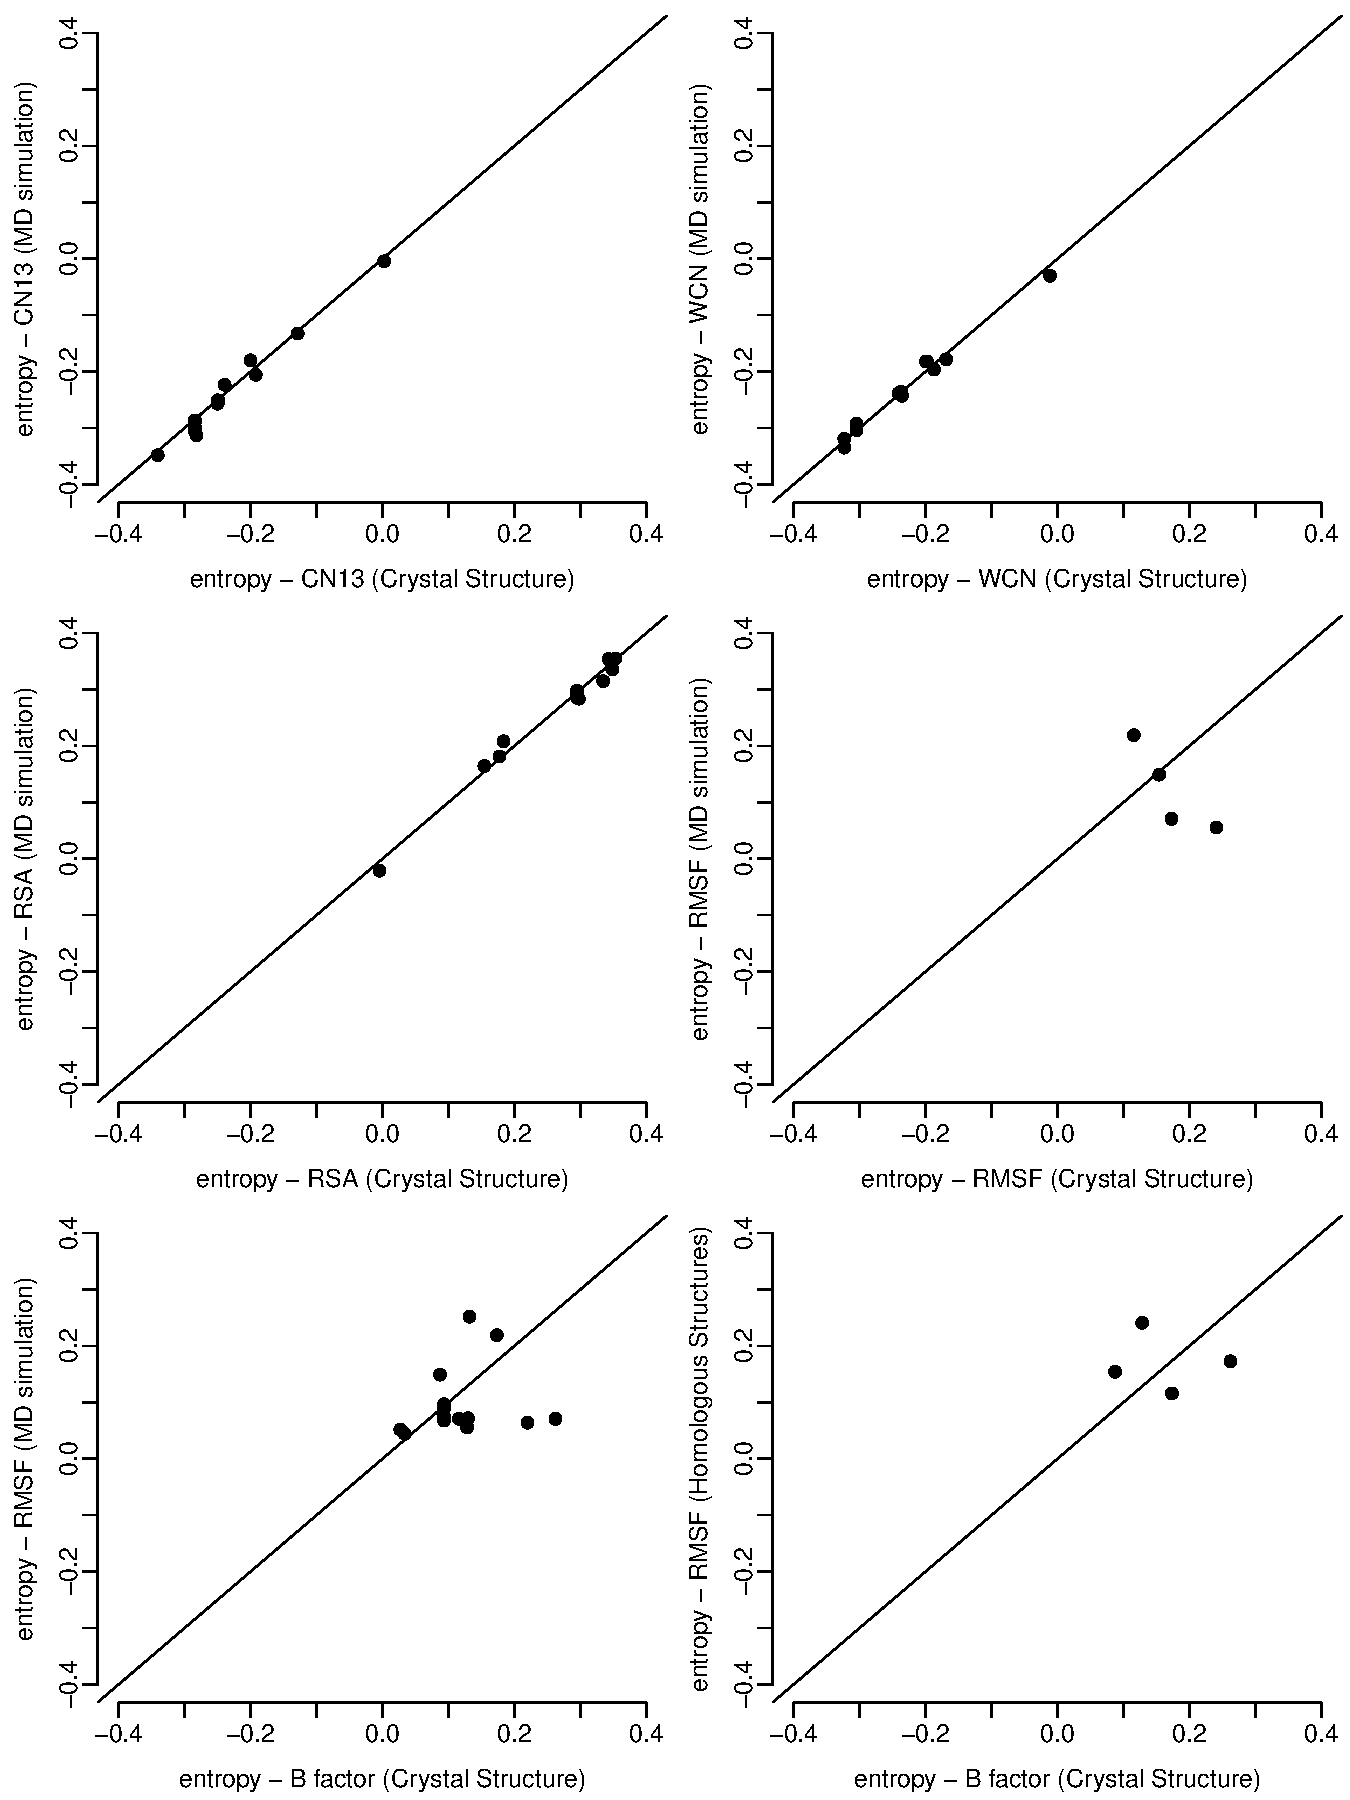
\includegraphics[height=0.7\textheight]{cor_cr_md.pdf}
            \end{center}
            \caption{
                     %{\bf Comparison of predictive power of four measures of structural variability about sequence entropy.}
                     {\bf Molecular dynamics vs. protein crystal structures in predicting sequence entropy.}
                     The vertical axes in all plots represent the Spearman's rank correlation coefficient of sequence entropy with one structural variable obtained from $15ns$ of Molecular Dynamics (MD) simulations. The horizontal axes represent the Spearman's rank correlation coefficient of sequence entropy with the same structural variable as in the vertical axes, but measured from protein crystal structures. Each black dot in the plots represents one protein structure provided in Table \ref{tab:pdb_names}. %The plots {\bf A}, {\bf B} \& {\bf C} all indicate the high similarity of the Relative Solvent Accessibility (RSA) and the two definitions of the amino acid Contact Number (ICN13 \& IWCN) measured from MD simulations with the corresponding measures from the protein crystal structures. Plot {\bf D} compares the correlation of sequence entropy with site-specific (backbone $C_\alpha$) Root-Mean-Square Fluctuation (RMSF) as measured from MD simulations and homologous crystal structures. Only four protein families had adequate number of homologous pdb structures for RMSF measurements to be included on this plot. Unlike measures of buriedness (RSA, ICN$13$ \& IWCN), RMSF from MD is not consistent with the corresponding measures from Crystal Structures. This is potentially due to the systematic biases that are involved in measuring RMSF (c.f., Section xx).
                     }
            \label{fig:cor_cr_md}
            \end{figure*}

            \begin{figure*}[t]
            \begin{center}
                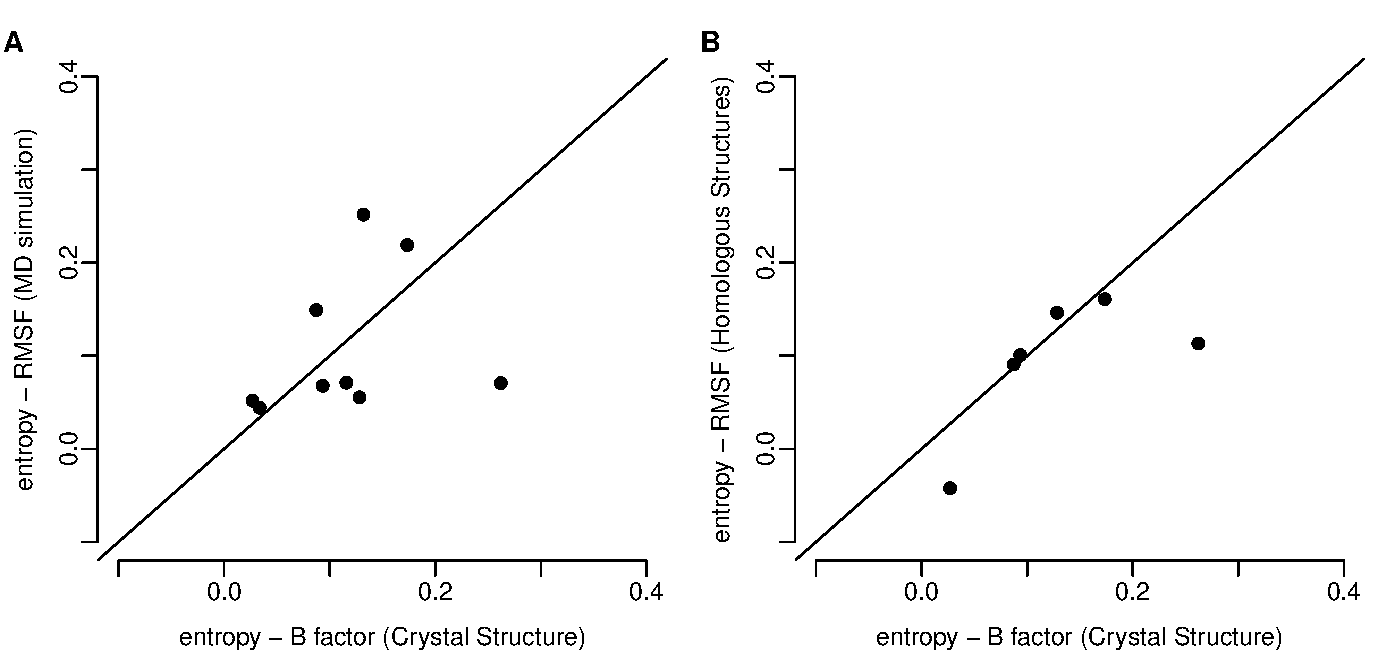
\includegraphics[height=0.35\textheight]{cor_entropy_bfca_rmsf.pdf}
            \end{center}
            \caption{
                     {\bf RMSF vs. B factor in sequence entropy prediction.} {\bf (A)} Comparison of the Spearman's rank correlation coefficients of entropy--RMSF with entropy-B factor. Each black dot represents one protein structure. {\bf (B)} Comparison of the Spearman's rank correlation coefficients of entropy--RMSF with entropy--B factor. Each black dot represents one protein structure for which there were adequate number of homologous structures in the Protein Data Bank, in order to calculate RMSF. As evidenced from the data in the plots, the three different measures of site-specific structural flexibility -- MD RMSF, CS RMSF, and B factor -- are inconsistent with each other.
                     }
            \label{fig:cor_entropy_bfca_rmsf}
            \end{figure*}

            \begin{figure*}[t]
            \begin{center}
                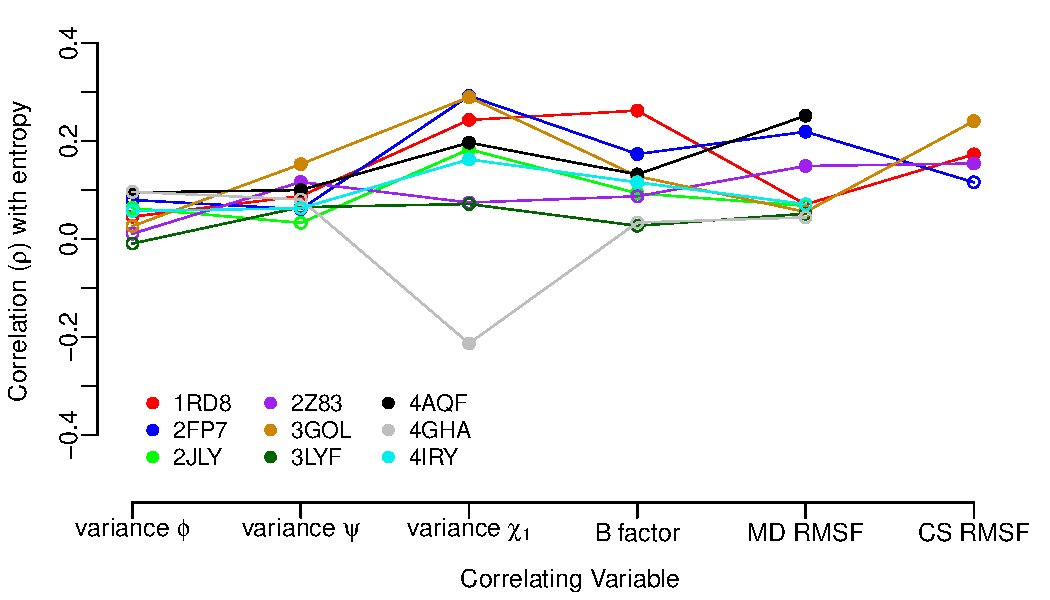
\includegraphics[height=0.35\textheight]{cor_entropy_SF.pdf}
            \end{center}
            \caption{
                     Comparison of the Spearman's rank correlation coefficients of different structural variability measures with sequence entropy. Different colors represent data for different protein PDB structures. The correlation coefficients are represented by solid dots where significant (i.e., $p$-value $\leq0.05$) or empty dots otherwise (where $p$-value $\geq0.05$). The variables $\phi$, $\psi$, and $\chi_1$ represent the protein's backbone dihedral angles, measured from MD simulations. The Root-Mean-Square Fluctuations for the proteins' $C_\alpha$ atoms are calculated from both MD simulations (variable MD RMSF) and Crystal Structures (CS RMSF). Almost all structural measures of variability correlate weakly, but significantly with sequence entropy.
                     }
            \label{fig:cor_entropy_SF}
            \end{figure*}
	
            \begin{figure*}[t]
            \begin{center}
                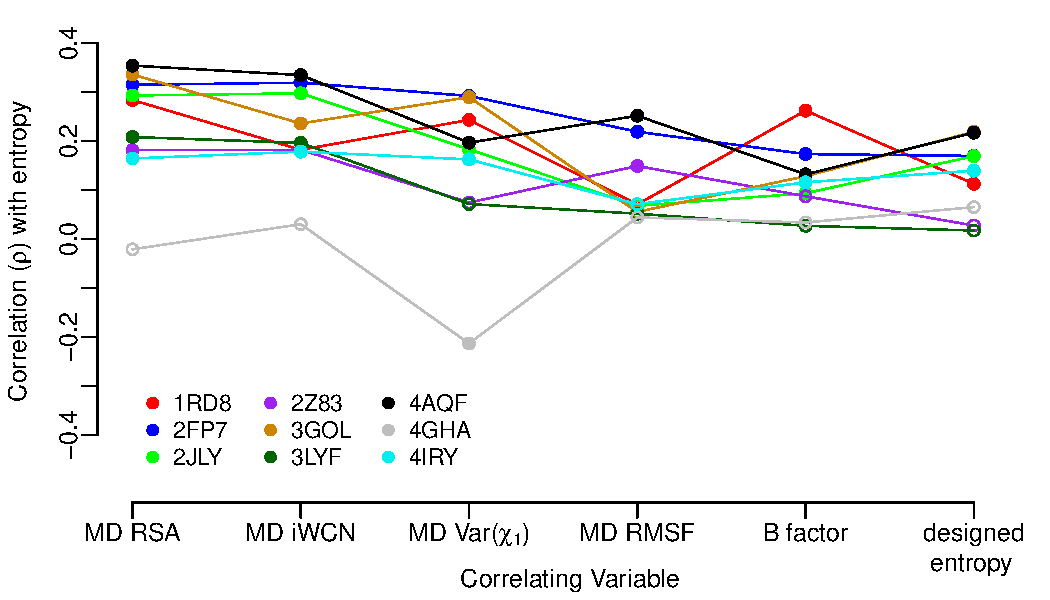
\includegraphics[height=0.35\textheight]{cor_entropy_all.pdf}
            \end{center}
            \caption{
                     Comparison of the Spearman's rank correlation coefficients of sequence entropy with structural variability and buriedness measures. Different colors represent data for different protein structures. The correlation coefficients are represented by solid dots where significant (i.e., $p$-value $\leq0.05$) or empty dots otherwise (where $p$-value $\geq0.05$). The variables: B factor, RMSF and the backbone dihedral angle $\chi_1$ represent different measures of structural variability and fluctuations, while the RSA and IWCN assess the amino acids solvent accessibility and the local packing density respectively. Compared to fluctuation measures, the buriedness variables consistently show stronger correlations with sequence entropy among all viral proteins considered in this analysis.
                     }
            \label{fig:cor_entropy_all}
            \end{figure*}

            \begin{figure*}[t]
            \begin{center}
                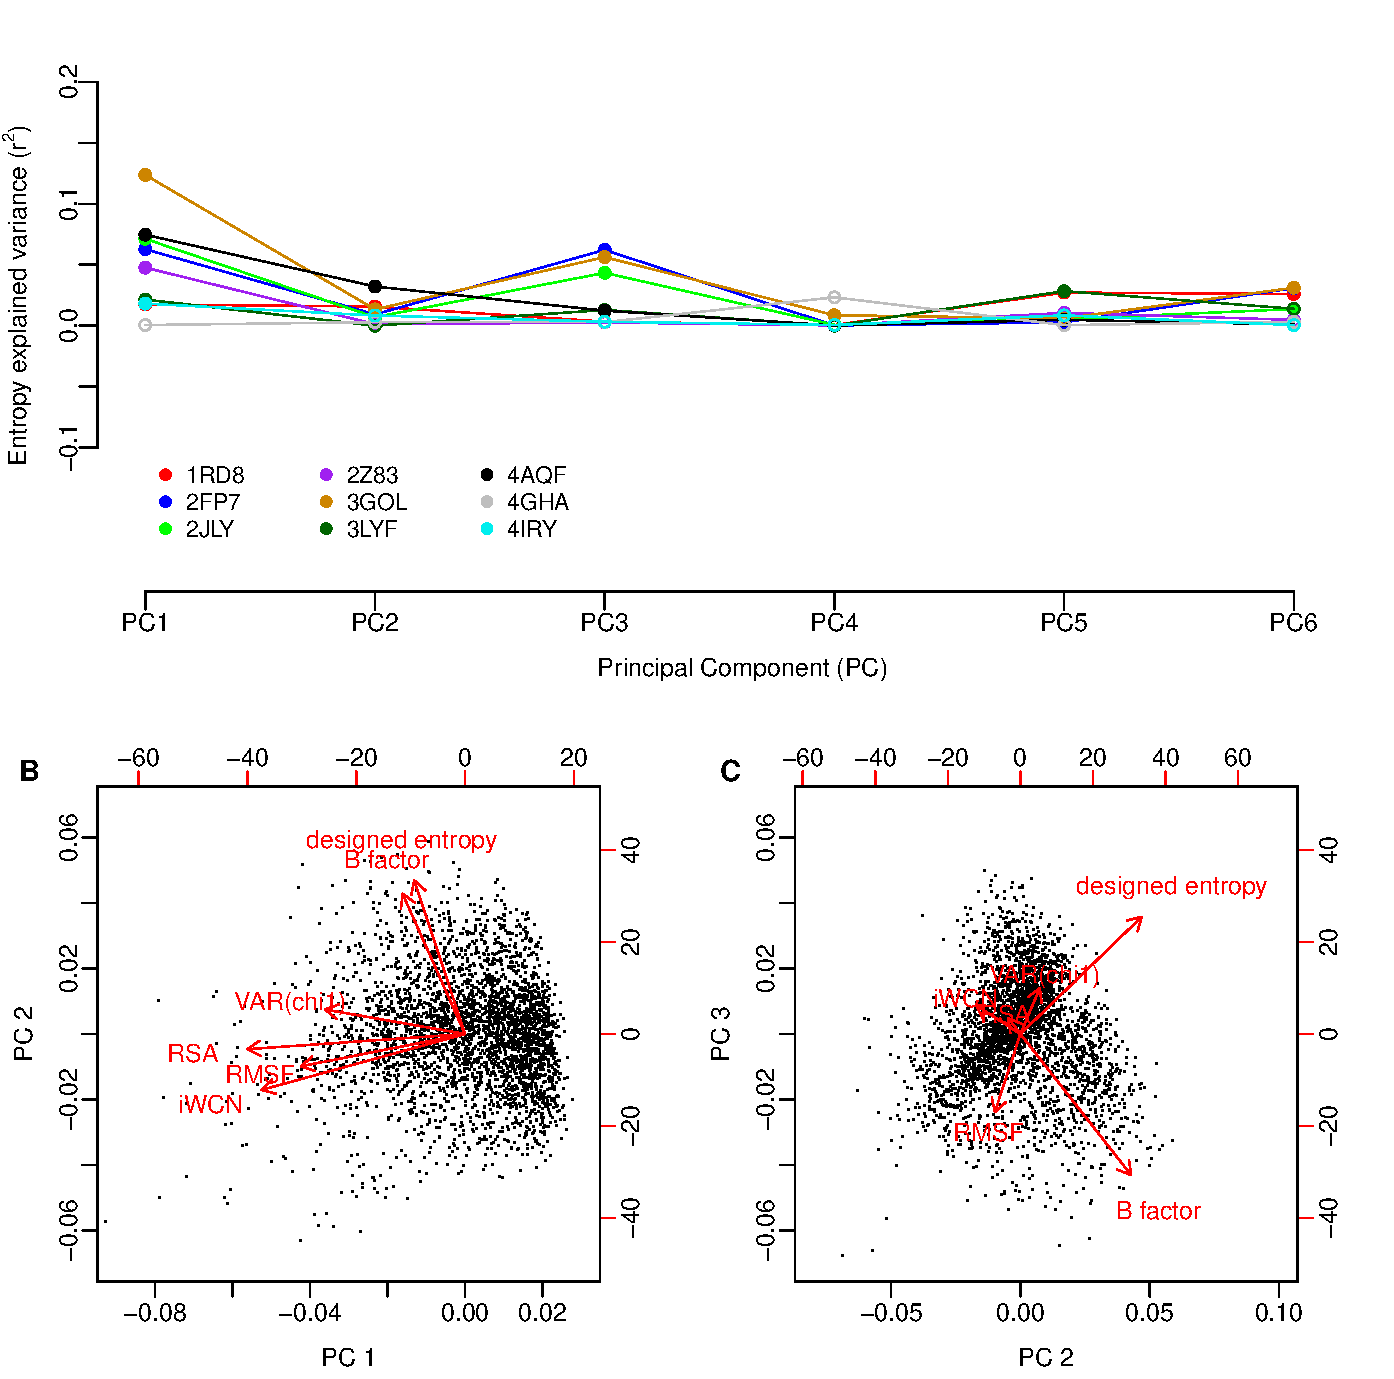
\includegraphics[height=0.7\textheight]{cor_entropy_PC_screen.pdf}
            \end{center}
            \caption{
                     {Principal Component (PC) Regression of sequence entropy given the structural variables:} {\bf (A)} An illustration of the Spearman's rank correlation coefficients of sequence entropy with different components of PC analysis on $6$ structural variability measures: RSA, iWCN, MD RMSF, B factor \& sequence entropy from designed proteins. Different colors represent data for different protein structures. The correlation coefficients are represented by solid dots where significant (i.e., $p$-value $\leq0.05$) or empty dots otherwise (where $p$-value $\geq0.05$). {\bf (B)} Plot of the second vs. first principal components depicting the major contribution of buriedness measures to the first component and therefore, to the explained variance of sequence entropy in plot {\bf (A)}. Red vectors represent the contributions of each of the structural variables to principal components and the black dots represent the amino acid sites on all $9$ protein structures considered. {\bf (C)} Plot of the third vs. first principal components depicting the major contribution of -- xx needs further discussion with Claus. I doubt if the original conclusion about these two plots is credible. xx
                     }
            \label{fig:cor_entropy_all}
            \end{figure*}

\input tab_pdb_names.tex


\end{document}


   with A high degree of similarity between the results from MD and CS is observed for RSA and the two definitions of contact number, WCN13 \& IWCN, with the exception of RMSF. The observed discrepancies between the two measures of RMSF from MD and crystal structures can possibly result from multiple factors: Insufficient length of molecular dynamics simulations, inherent biases that exist in the definition of RMSF, and finally, the potential lack of an intrinsic association between RMSF and sequence entropy.
         The lack of consistency between the three independent measures of structural fluctuations together with the overall weak, though positive, correlations of these measures with sequence entropy again points to the potential existing biases in the definition and measurement of these variables.
